\chapter{System Overview}

The system consists of three core components: a camera module, a microcontroller-based processing unit, and a user-interfacing application connected via a network. The camera module used is the Arducam Mega 3MP, which interfaces with the STM32L475 IoT Discovery Kit (DISCO\_L475\_IOT1) over the SPI bus. The microcontroller board then communicates with a remote TCP server using its built-in Wi-Fi module. A mobile application acts as the user interface to the system. The overall hardware architecture is depicted in Fig.~\ref{overall}.

\begin{figure}[h!]
  \centering
  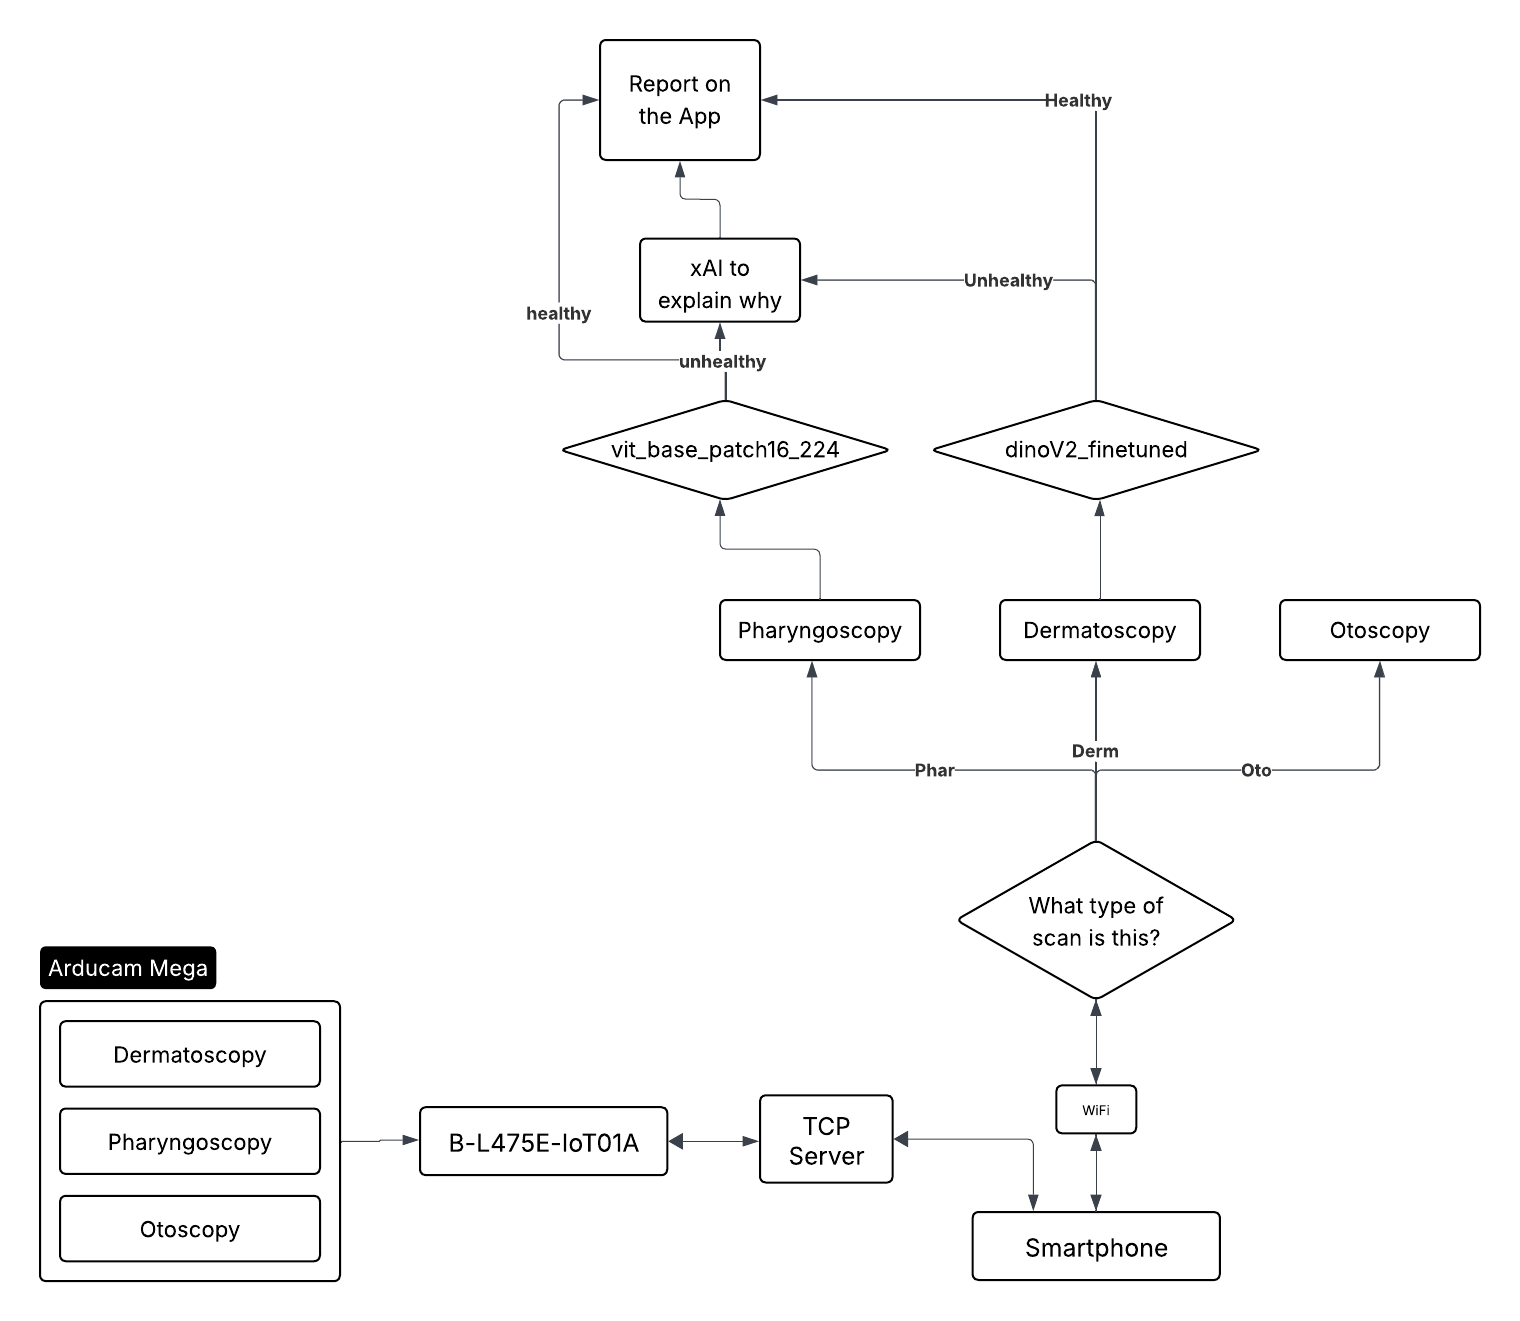
\includegraphics[width=0.8\linewidth]{system_diagram.png}
  \caption{Block diagram of the complete system.}
  \label{overall}
\end{figure}

\section{Camera Selection}

To obtain sufficiently accurate results from the AI model used for image analysis, a minimum image resolution of 1080p is required. This resolution ensures that key visual features are preserved and detectable, allowing the AI algorithms to perform accurate classification, detection, or segmentation tasks. Although the Arducam Mega 3MP does not strictly provide 1920$\times$1080 resolution (1080p), it offers a maximum resolution of approximately 2048$\times$1536, which exceeds the 1080p requirement. Therefore, it satisfies the minimum resolution threshold for AI processing while maintaining a compact form factor and low power requirements suitable for embedded systems.

\section{Microcontroller Platform}

The STM32L475 IoT Discovery Kit was chosen for its low-power ARM Cortex-M4 microcontroller and the wide range of onboard sensors and communication modules, including Wi-Fi, Bluetooth, and NFC. This makes it an ideal platform for rapid prototyping of IoT applications. Its power efficiency is crucial for battery-powered or energy-constrained scenarios, and the board provides enough processing capability to handle real-time interfacing with the camera and network communication tasks.

\section{RTOS Selection: Zephyr}

The firmware for the STM32L475 is developed using the Zephyr RTOS. Zephyr is a scalable, real-time operating system designed specifically for resource-constrained embedded devices. It provides a rich set of features such as multithreading, device drivers, and networking stacks, which are essential for handling the simultaneous operations of camera control, SPI communication, and Wi-Fi networking. Its modular architecture allows developers to include only the necessary components, keeping the firmware lightweight and efficient. Additionally, Zephyr supports a wide range of boards and peripherals, easing development and maintenance.

\section{Communication Protocol: TCP}

TCP was selected as the communication protocol between the microcontroller and the server due to its reliability. Unlike UDP, TCP provides guaranteed delivery, in-order packet transmission, and error checking, which are essential for transmitting critical data such as images and camera configuration commands. While TCP introduces slightly more overhead than UDP, its robustness outweighs this cost, especially in use cases where data integrity and reliable communication are paramount. The use of TCP ensures that image data is transmitted accurately to the server without loss or corruption.

